Na rys.~\ref{fig:2} przedstawiono wyniki
eksperymentu~\ref{subsec:rhodobacter}.
W 10 dniu eksperymentu widoczny jest istotny
statystycznie spadek OD\textsubscript{600}
w próbkach o $c_{WW} = 80$ \% względem próbek
o niższych stężeniach.
Oznacza to hamowanie wzrostu \textit{R. spheroides}
przy stężeniach WW 80 \%.
Z~tego względu w kolejnych eksperymentach kultywowano
\textit{R. spheroides} na M27 + 50 \% WW\@.
Rys.~\ref{fig:3} przedstawia wyniki
eksperymentu~\ref{subsec:mlra}.
(\ldots)
Na rys.~\ref{fig:4} przedstawiono wyniki pomiarów
napięcia w eksperymencie~\ref{subsec:volt}.
Z wykresu wynika, że największe napięcia generowane
są w przypadku hodowli \textit{R. spheroides}
o OD\textsubscript{600} w zakresie od 0.200 do 0.535,
przy czym hodowle gęstsze, o~OD\textsubscript{600} bliskim
0.500 wykazują spadki napięcia po dłuższym czasie.

\begin{figure}[t]
    \centering
    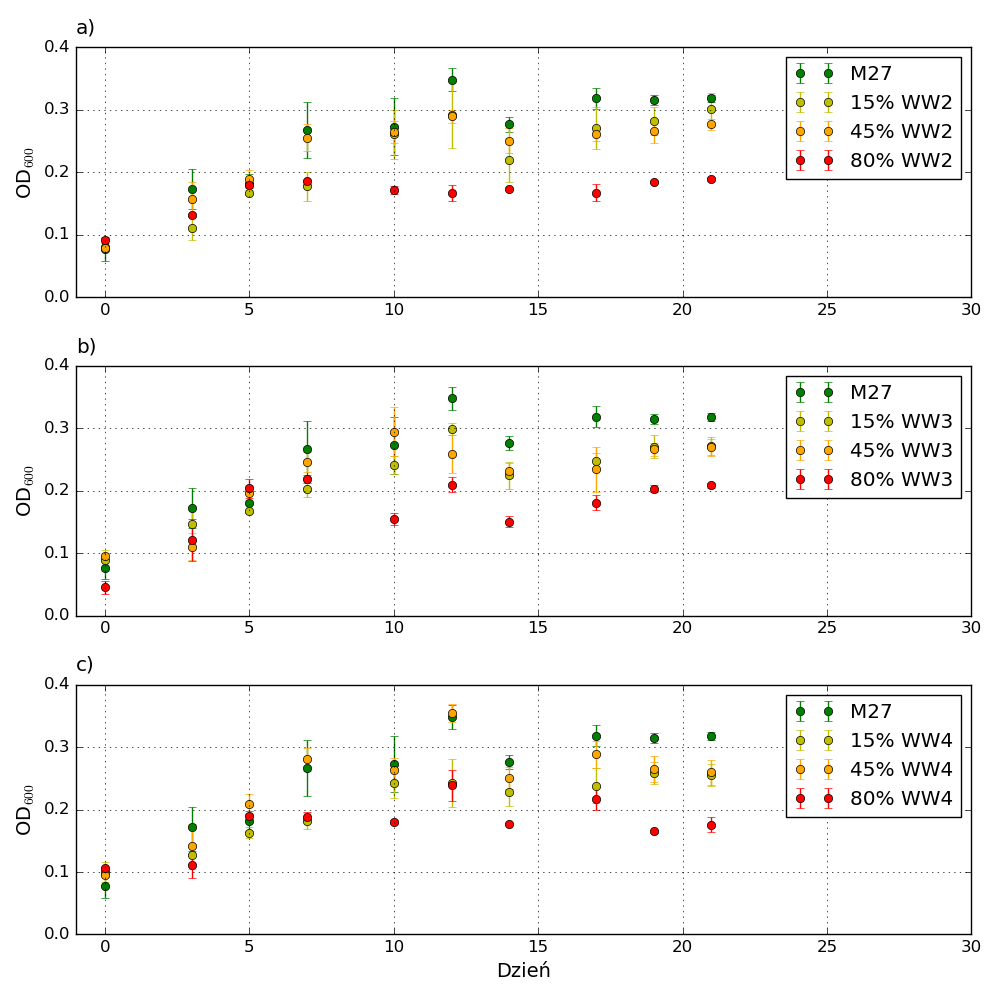
\includegraphics[width=14cm]{figures/ww}
    \caption{
        Zmiany OD\textsubscript{600} hodowli \textit{R. spheroides} w czasie w M27:
        a)~zawierającym WW2 w~stężeniach 15 \%, 45 \% i 80 \%;
        b)~zawierającym WW3 w stężeniach 15 \%, 45 \% i 80 \%;
        c)~zawierającym WW4 w stężeniach 15 \%, 45 \% i 80 \%.
        Słupki błędów to SEM (n = 3).
    }
    \label{fig:2}
\end{figure}

\begin{figure}
    \centering
    \includegraphics[width=12cm]{}
    \caption{
        Aktywność MlrA w lizatach komórek
        \textit{Synechocystis sp.} PCC 6803 McCormick 7
        kultywowanych z użyciem różnych rodzajów i stężeń WW
        w BG-11 jako pożywki. Słupki błędów to SEM (n = 3).
    }
    \label{fig:3}
\end{figure}

\begin{figure}
    \centering
    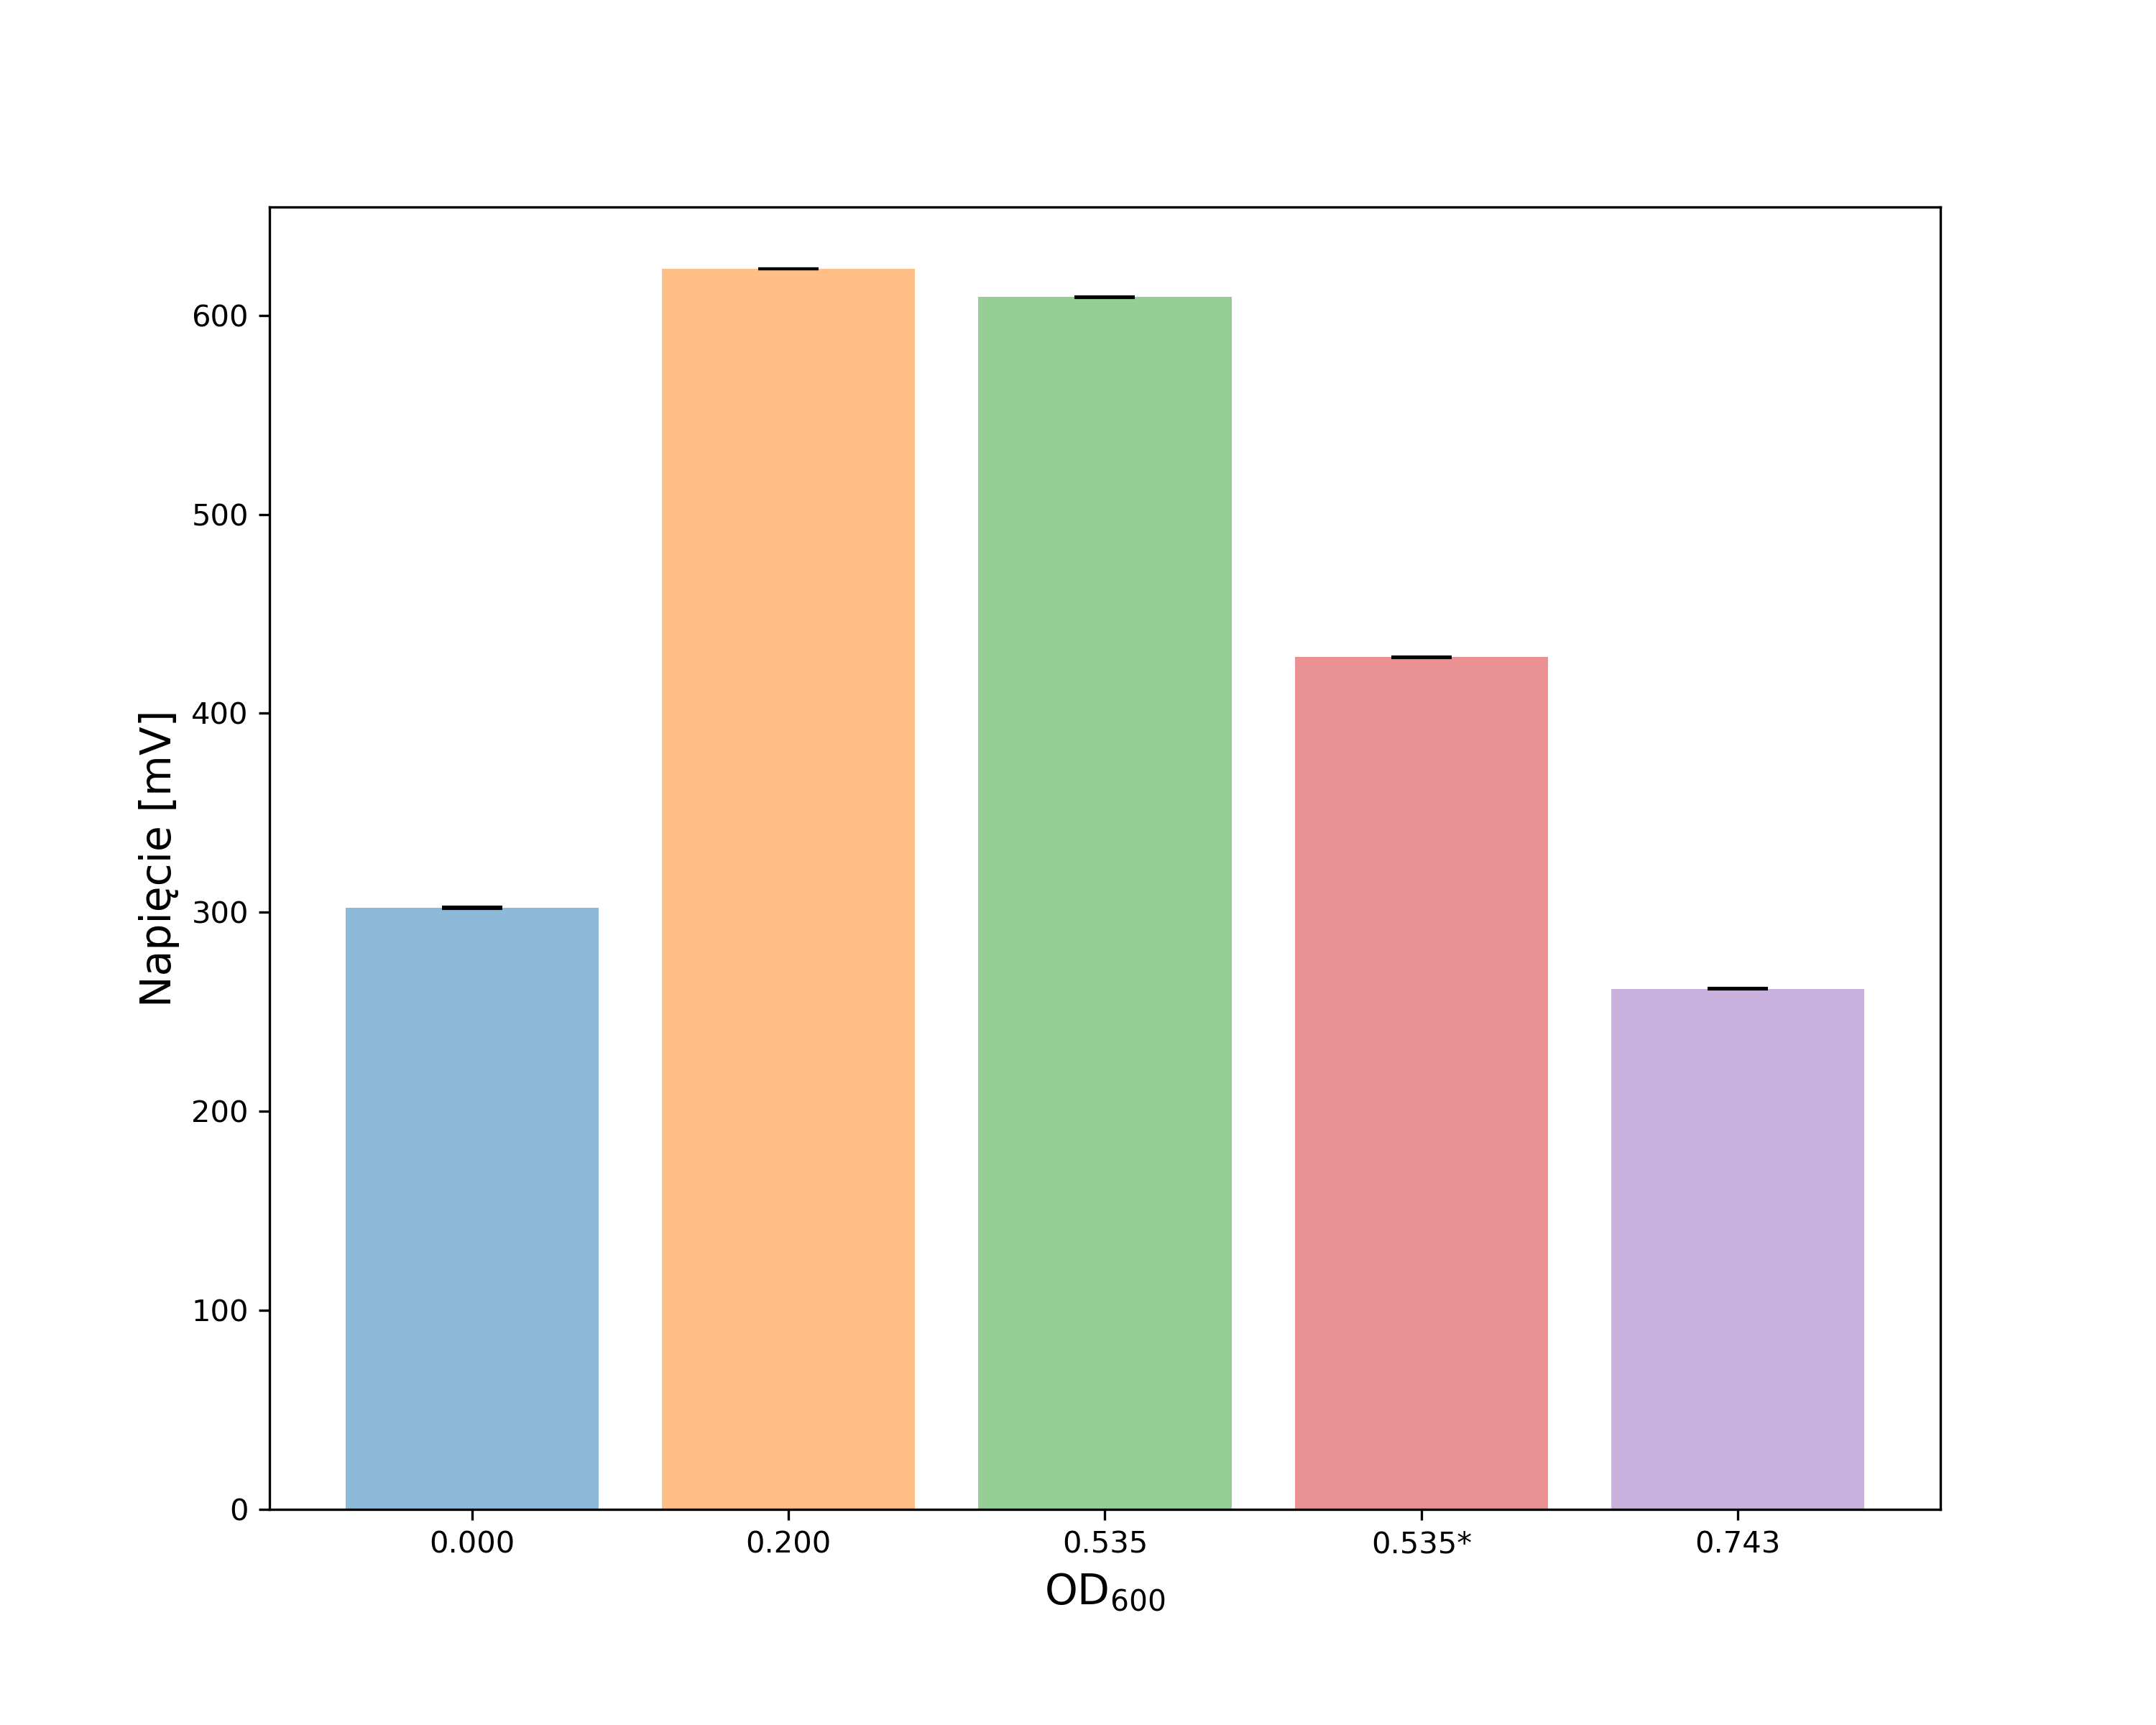
\includegraphics[width=12cm]{figures/voltage3}
    \caption{
        Uśrednione wartości napięcia w zależności od OD\textsubscript{600}
        hodowli \textit{R. spheroides} znajdującej się w komorze z anodą.
        *Pomiar wykonany po 24 h adaptacji mikroorganizmów do elektrody.
        Słupki błędów to SEM (n = 11; dla OD\textsubscript{600} = 0.743, n = 8).
    }
    \label{fig:4}
\end{figure}
